\section{Scheduling bij één processor}

Een besturingssysteem moet bronnen toewijzen tussen wedijverende processen. De processor biedt als bron aan uitvoeringstijd. De bron is toewijsbaar in betekenis van inroosteren.

Het doel van processor scheduling is het toewijzen van processen die uitgevoerd moeten worden door de processor over een bepaalde tijdsperiode op een manier dat het de systeem objectieven voldaan zijn, zoals response tijd, doorvoersnelheid en efficiënt gebruik van de processor.

De scheduling functie zou moeten voldoen aan volgende zaken:

\begin{itemize}
\item De tijd moet eerlijk verdeeld zijn tussen processen
\item Het moet voorkomen dat een proces aan uithongering (starvation) lijdt
\item De processor moet efficiënt gebruikt worden
\item Er moet lage overhead zijn
\item Processen moeten een hogere prioriteit krijgen indien nodig 
\end{itemize}

Typen scheduling/

\textbf{Scheduling voor lange termijn (long-term scheduling) =}	De beslissing een proces toe te voegen aan de verzameling processen die worden uitgevoerd

\textbf{Scheduling voor middellange termijn (medium-term scheduling) =}	De beslissing een proces toe te voegen aan de processen die zich gedeeltelijk of geheel in het hoofdgeheugen bevinden.

\textbf{Scheduling voor korte termijn (short-term scheduling) =}	De beslissing welk beschikbare proces zal worden uitgevoerd door de processor

\textbf{I/O scheduling =}	De beslissing welk openstaan I/O-verzoek van een apparaat zal worden afgehandeld door een beschikbaar I/O-apparaat.

\subsection{Soorten scheduling}

\begin{figure}[htp]
    \centering
            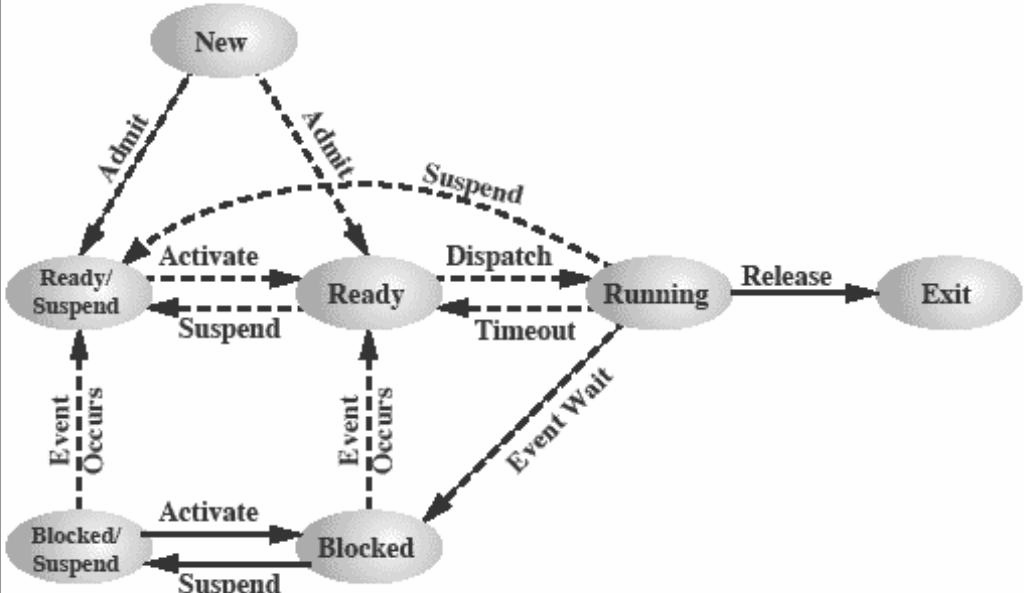
\includegraphics[width=4in]{img/overgangsmodelvoorprocestoestanden.png}
        \caption{Oud schema hoofdstuk 3 (overgangsmodel voor procestoestanden)}
    \label{fig:Oud schema hoofdstuk 3 (overgangsmodel voor procestoestanden)}
\end{figure}

\begin{figure}[htp]
    \centering
            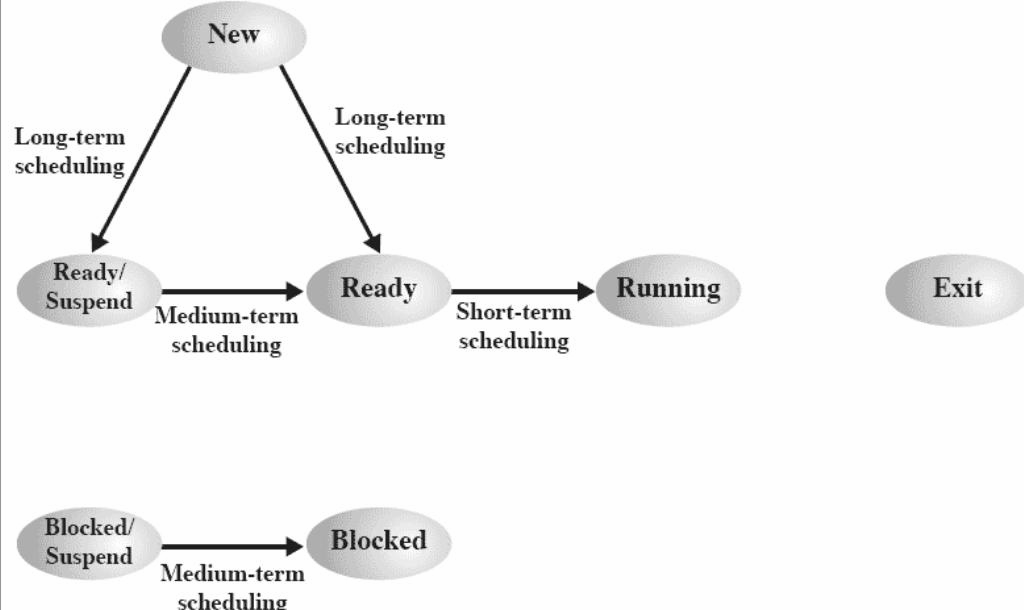
\includegraphics[width=4in]{img/schedulingsfuncties.png}
        \caption{De relatie tussen de schedulingfuncties en het overgangsmodel voor procestoestanden}
    \label{fig:De relatie tussen de schedulingfuncties en het overgangsmodel voor procestoestanden}
\end{figure}

\begin{figure}[htp]
    \centering
            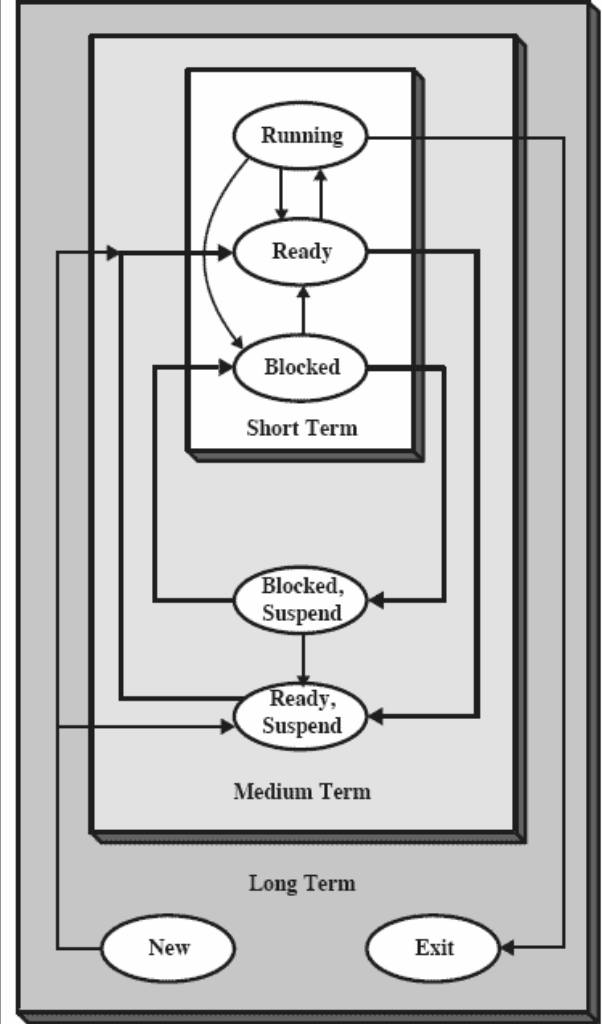
\includegraphics[width=4in]{img/samenhangschedulingfuncties.png}
        \caption{De interne samenhang van de schedulingfuncties}
    \label{fig:De interne samenhang van de schedulingfuncties}
\end{figure}

\begin{figure}[htp]
    \centering
            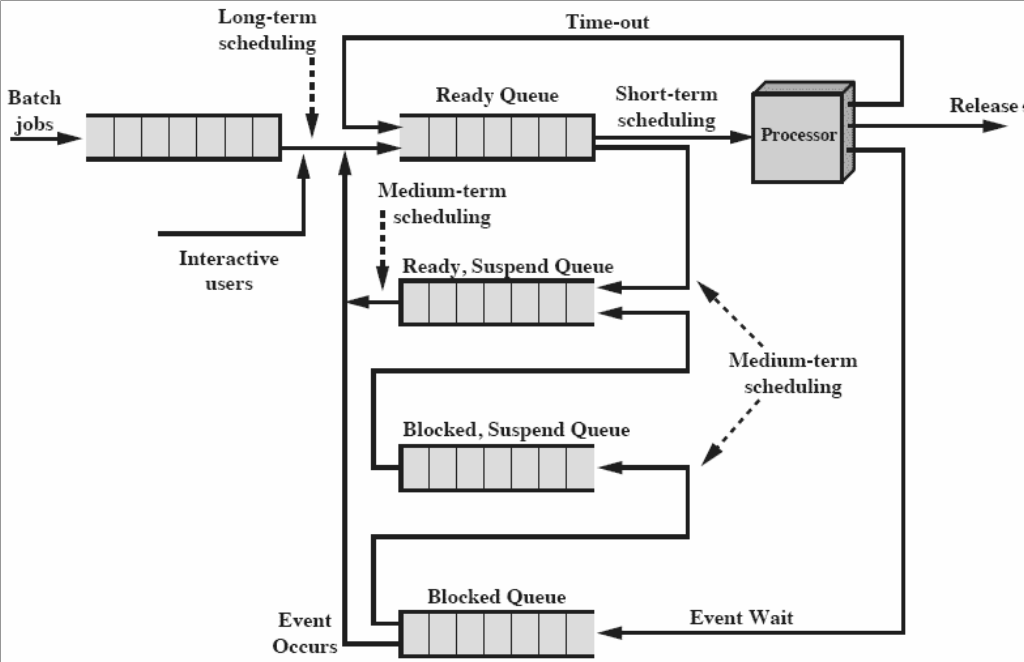
\includegraphics[width=4in]{img/invloedscheduling.png}
        \caption{Hoe scheduling de prestaties van het systeem beïnvloedt omdat scheduling bepaalt welke processen wachten en welke processen worden voortgezet}
    \label{fig:Hoe scheduling de prestaties van het systeem beïnvloedt omdat scheduling bepaalt welke processen wachten en welke processen worden voortgezet}
\end{figure}

\subsubsection{Scheduling voor lange termijn}

Long-term scheduling bepaalt welke programma’s worden toegelaten tot het systeem voor verwerking.

Kan zijn First-come-first-served. OF kan aan de hand van prioriteiten, I/O-benodigdheden of verwachte uitvoeringstijd.

Het controleert het niveau van multiprogramming.

Hoe meer processen, hoe kleiner het percentage tijd dat elk proces krijgt voor uitvoering.


\subsubsection{Scheduling voor middellange termijn. Dit is deel van de swapping functie.}

Swapping-in beslissingen zijn gebaseerd op de noodzaak om de mate van multiprogramming te beheren.

\subsubsection{Scheduling voor korte termijn}

Dit is gekend als de dispatcher. Wordt het meest uitgevoerd.

Wordt geactiveerd wanneer bepaalde gebeurtenissen plaatsen vinden:

\begin{itemize}
\item Klok interrupts
\item I/O interrupts
\item Besturingssysteemaanroepen
\item Signalen
\end{itemize}